%% LaTeX Template for ISIT 2019
%%
%% by Stefan M. Moser, October 2017
%% 
%% derived from bare_conf.tex, V1.4a, 2014/09/17, by Michael Shell
%% for use with IEEEtran.cls version 1.8b or later
%%
%% Support sites for IEEEtran.cls:
%%
%% http://www.michaelshell.org/tex/ieeetran/
%% http://moser-isi.ethz.ch/manuals.html#eqlatex
%% http://www.ctan.org/tex-archive/macros/latex/contrib/IEEEtran/
%%

\documentclass[conference,letterpaper]{IEEEtran}

%% depending on your installation, you may wish to adjust the top margin:
\addtolength{\topmargin}{9mm}

%%%%%%
%% Packages:
%% Some useful packages (and compatibility issues with the IEEE format)
%% are pointed out at the very end of this template source file (they are 
%% taken verbatim out of bare_conf.tex by Michael Shell).
%
% *** Do not adjust lengths that control margins, column widths, etc. ***
% *** Do not use packages that alter fonts (such as pslatex).         ***
%
\usepackage[utf8]{inputenc} 
\usepackage[T1]{fontenc}
\usepackage{url}
\usepackage{ifthen}
\usepackage{cite}
\usepackage[cmex10]{amsmath} % Use the [cmex10] option to ensure complicance
\usepackage{amssymb, amsthm}
\usepackage{mathtools}
\usepackage{xfrac}
\usepackage{svg}
\usepackage{graphicx}
\usepackage{cleveref}
\newcommand{\subparagraph}{}
\usepackage{titlesec}
                             % with IEEE Xplore (see bare_conf.tex)

%% Please note that the amsthm package must not be loaded with
%% IEEEtran.cls because IEEEtran provides its own versions of
%% theorems. Also note that IEEEXplore does not accepts submissions
%% with hyperlinks, i.e., hyperref cannot be used.

\interdisplaylinepenalty=2500 % As explained in bare_conf.tex
\newtheorem{theorem}{Theorem}
\newtheorem{lemma}[theorem]{Lemma}
\newtheorem{corollary}[theorem]{Corollary}
\newtheorem{claim}[theorem]{Claim}
\newtheorem{proposition}[theorem]{Proposition}
\newtheorem{remark}{Remark}
\newtheorem{definition}{Definition}
\newtheorem{example}{Example}
\newtheorem{exercise}{Exercise}
%%%%%%
% correct bad hyphenation here
\hyphenation{op-tical net-works semi-conduc-tor}

\titlespacing*{\subsection}
  {0pt}{0 mm}{0 mm}
\titlespacing*{\section}
  {0pt}{2 mm}{1 mm}
\crefname{equation}{}{}
% ------------------------------------------------------------
\begin{document}
\title{A method to find the volume of a sphere in the Lee metric, and its applications} 

%%% Single author, or several authors with same affiliation:
 \author{%
   \IEEEauthorblockN{Sagnik Bhattacharya, Adrish Banerjee}
   \IEEEauthorblockA{Department of Electrical Engineering, Indian Institute of Technology Kanpur\\
                     Email: \{sagnikb, adrish\}@iitk.ac.in}
  %\and
  %\IEEEauthorblockN{Adrish Banerjee}
   %\IEEEauthorblockA{Professor\\
                     %IIT Kanpur\\
                     %Kanpur, India\\
                     %Email: adrish@iitk.ac.in}
 }


%%% Several authors with up to three affiliations:
%\author{%
%  \IEEEauthorblockN{Stefan M.~Moser}
%  \IEEEauthorblockA{ETH Zürich\\
%                    ISI (D-ITET), ETH Zentrum\\
%                    CH-8092 Zürich, Switzerland\\
%                    Email: moser@isi.ee.ethz.ch}
%  \and
%  \IEEEauthorblockN{Albus Dumbledore and Harry Potter}
%  \IEEEauthorblockA{Hogwarts School of Witchcraft and Wizardry\\
%                    Hogwarts Castle\\ 
%                    1714 Hogsmeade, Scotland\\
%                    Email: \{dumbledore, potter\}@hogwarts.edu}
%}


%%% Many authors with many affiliations:
% \author{%
%   \IEEEauthorblockN{Albus Dumbledore\IEEEauthorrefmark{1},
%                     Olympe Maxime\IEEEauthorrefmark{2},
%                     Stefan M.~Moser\IEEEauthorrefmark{3}\IEEEauthorrefmark{4},
%                     and Harry Potter\IEEEauthorrefmark{1}}
%   \IEEEauthorblockA{\IEEEauthorrefmark{1}%
%                     Hogwarts School of Witchcraft and Wizardry,
%                     1714 Hogsmeade, Scotland,
%                     \{dumbledore, potter\}@hogwarts.edu}
%   \IEEEauthorblockA{\IEEEauthorrefmark{2}%
%                     Beauxbatons Academy of Magic,
%                     1290 Pyrénées, France,
%                     maxime@beauxbatons.edu}
%   \IEEEauthorblockA{\IEEEauthorrefmark{3}%
%                     ETH Zürich, ISI (D-ITET), ETH Zentrum, 
%                     CH-8092 Zürich, Switzerland,
%                     moser@isi.ee.ethz.ch}
%   \IEEEauthorblockA{\IEEEauthorrefmark{4}%
%                     National Chiao Tung University (NCTU), 
%                     Hsinchu, Taiwan,
%                     moser@isi.ee.ethz.ch}
% }


\maketitle

%%%%%%
%% Abstract: 
%% If your paper is eligible for the student paper award, please add
%% the comment "THIS PAPER IS ELIGIBLE FOR THE STUDENT PAPER
%% AWARD." as a first line in the abstract. 
%% For the final version of the accepted paper, please do not forget
%% to remove this comment!
%%
\begin{abstract}
  We develop general techniques to bound the size of the balls of a given radius $r$ for $q$-ary discrete metrics, using the generating function for the metric and Sanov's theorem, that reduces to the known bound in the case of the Hamming metric and gives us a new bound in the case of the Lee metric. We use the techniques developed to find Hamming, Elias-Bassalygo and Gilbert-Varshamov bounds for the Lee metric. 
\end{abstract}


%% The paper must be self-contained. However, if you are referring to
%% a full version for checking certain proofs, please provide the
%% publically accessible location below.  If the paper is completely
%% self-contained, you can remove the following line from your
%% submission.

\section{Introduction}
\subsection{Background}
One of the outcomes of Shannon's classic work on information theory is a long and ongoing investigation of point-to-point communication over a discrete memoryless channel and the limits of reliable communication over such a channel. To describe these limits, we can use various metrics defined on the codeword space that are matched to the channel under consideration, where we say that a metric is matched to a channel if nearest neighbour decoding according to the metric implies maximum likelihood (ML) decoding on the channel \cite{lee}. The kind of metric chosen can vary, for example, depending on the kind of modulation scheme used for communication over the channel. The limits also change depending on what kind of error criterion is being used - for example, whether we want average error or maximum error to be bounded.

The most well studied metric is the Hamming metric, which is suited to orthogonal modulation schemes \cite{Berlekamp:2015:ACT:2834146}. For the error rate to be exactly zero, we have several upper bounds like the low-rate average-distance Plotkin bound \cite{hamplotkin}, the Hamming bound based on sphere packing \cite{Berlekamp:2015:ACT:2834146}, the Elias-Bassalygo bound\cite{EBbound} and the linear programming based MRRW bound\cite{MRRW}, and lower bounds like the Gilbert-Varshamov bound \cite{gv1}  that tell us what rates are possible and what are not, given an error criterion that the code is to meet, even though the question of what is the precise capacity is still open. Many of these bounds use at some point a bound on the number of codewords of length $n$ of a certain $q$-ary Hamming weight $r$, which is the size of the Hamming ball of radius $r$, and the standard known result is that this size is $q^{nH_q(r/n)}$ to first order in the exponent, where $H_q(\cdot)$ is the $q$-ary entropy function. 

There are other metrics of practical and mathematical interest, for example the Lee metric, introduced in \cite{Lee1958SomePO, ulrich}. This metric is known to be suited to phase modulation schemes \cite{Berlekamp:2015:ACT:2834146}, and has more recently been used in multi-dimensional burst-error correction \cite{bursts}, error correction for flash memories \cite{flash},   interleaving schemes\cite{interleaving}, and constrained and partial response channels \cite{roth-siegel}.

\subsection{Prior work}
Given a bound on the volume of the $q$-ary Lee ball of radius $t$, $V_{t}^{(n)}$, for a code of blocklength $n$, Chiang and Wolf \cite{lee} give the Hamming bound 
\begin{equation}\label{Hamming bound}
    V_{(d-1)/2}^{(n)} \leq q^{n(1-R(d))}
\end{equation}
and the Gilbert-Varshamov bound, 
\begin{equation}\label{GV bound}
    V_{d}^{(n)} > q^{n(1-R(d))}
\end{equation}
on the rate $R(d)$ for a code of minimum distance $d$ in the Lee metric. They also give the following bound analogous to the singleton bound for a linear code of length $n$ and rank $k$ in the Lee metric,
\begin{equation}
    d \leq  
    \begin{cases}
        \frac{q+1}{4}(n-k+1) & \text{for odd $q$}\\
        \frac{q^2}{4(q-1)}(n-k+1) & \text{for even $q$} \\
    \end{cases}
\end{equation}
and the following method of calculating the volume of a sphere in the Lee metric
\begin{equation}
    V_r^{(n)} (z) = \left(\sum_{i = 0}^{r} \frac{1}{i!}\frac{d^i}{dz^i} A^{(n)} (z)\right)_{z = 0}
\end{equation}
which is mathematically involved. Here $A^{(n)} (z)$ is the generating function for the Lee metric.

Wyner and Graham \cite{DBLP:journals/iandc/WynerG68} give the following Plotkin-type bound for the Lee metric:
$
    d \leq \frac{n \overline{D}}{1 - \lvert C \rvert^{-1}}
$
where 
\begin{equation}
    \overline{D} =  
    \begin{cases}
        \frac{q^2-1}{4q} & \text{for odd $q$}\\
        \frac{q}{4} & \text{for even $q$} \\
    \end{cases}
\end{equation}
and $\lvert C \rvert$ is the size of the code.
Berlekamp \cite{Berlekamp:2015:ACT:2834146} used a result due to Chernoff \cite{chernoff1952} to find the volume of a ball in the Hamming metric using the generating function as a starting point, but omits the corresponding calculations for the Lee metric as they are too tedious. He also gives a version of the Elias-Bassalygo bound for $0 < t < \overline{D}n$:
\begin{equation}
    d \leq \left(\frac{t}{1-K^{-1}}\right)\left(2 - \frac{t}{n\overline{D}}\right)
\end{equation}
where $K$ is the least integer not less than $\frac{V_t^{(n)}}{q^{n(1-R)}}$, and $t$ is chosen to minimize the RHS of the inequality.

Golomb \cite{golomb} gave several results on spheres in several different discrete metrics.

Roth \cite{Roth:2006:ICT:1137784} also gives versions of the Hamming and Gilbert-Varshamov bounds for the Lee metric, and gives the following closed form expression for the volume of a Lee sphere of radius $t < \frac{q}{2}$ (here $\binom{t}{i} = 0$ if $i > t$).
\begin{equation}
    V_{t}^{(n)} = \sum_{i = 0}^{n}2^i \binom{n}{i} \binom{t}{i}
\end{equation}

As an exercise, he also includes the result that his expression is a strict lower bound for all $t \geq \frac{q}{2}$.

\subsection{Our contributions}
We develop a general technique based on the generating function of a metric and Sanov's theorem to find the volume of a sphere of a given radius. We show that this method allows us to recover the familiar bounds on the volume of a Hamming ball. We find upper and lower bounds on the volume of a ball in the Lee metric, and we use this result to find bounds analogous to the Hamming, Elias-Bassalygo and Gilbert-Varshamov bounds for the Lee metric.

\subsection{Structure of the paper}
In \cref{setup}, we introduce the necessary notation. In \cref{general method} we describe the general method using Sanov's theorem, and we give specific examples of it's use in \cref{examples} -  the Hamming metric in \cref{hamming example} and the Lee metric in \cref{lee metric}. Finally, in \cref{Lee metric bounds}, we use the results developed in the \cref{lee metric} to find Hamming and Gilbert-Varshamov bounds for the Lee metric.

\section{Problem Setup and Notation}\label{setup}
    We adopt a slightly modified version of the notation and terminology of Berlekamp\cite{Berlekamp:2015:ACT:2834146}. The discrete metric under consideration gives the distance between any two points in the space of $n$-length vectors over an alphabet of $q$ symbols. Given a center $C$ and a radius $r$, define the sphere $\mathcal{S}(C,t)$ as the set of all points whose distance from $C$ is less than or equal to $t$. The surface area of such a sphere is the number of vectors whose distance from $C$ is exactly $t$ and it is denoted by $A_t^{(n)}$. The volume of such a sphere is the number of vectors whose distance from $C$ is $\leq t$, and it is denoted as $V_t^{(n)}$. Clearly, we have the equality $V_t^{(n)} = \sum_{j = 0}^t A_j^{(n)}$. Now, let $A^{(n)}(z) = \sum_{j} A_j^{(n)} z^j$, the generating function for the $A_j^{(n)}$. Since the distance is additive over the $n$ coordinates, the generating function is multiplicative over these coordinates, and we have the equality $A^{(n)}(z) = [A^{(1)}(z)]^n$, where $A^{(1)}(z)$ gives the weights for a single symbol only. For example, for the Hamming metric we have $A^{(1)}(z) = 1 + (q-1)z$, and for the Lee metric we have
    \begin{equation}
        A^{(1)}(z) = 
            \begin{cases}
                1 + 2z + 2z^2 + \ldots + 2z^{\frac{q-1}{2}} & \text{for odd $q$} \\
                1 + 2z + 2z^2 + \ldots + 2z^{\frac{q-2}{2}} + z^{\frac{q}{2}} & \text{for even $q$} \\
            \end{cases}
    \end{equation}
    
\section{The general method}\label{general method}
We now describe a generalised method that works for any metric before going into specific examples. For any $A^{(1)}(z)$, we get a random variable $X$ as follows: if $A^{(1)}(z)$ contains a term of the form $\alpha(j)z^i$, then the random variable $X$ takes value $j$ with probability $\frac{\alpha(j)}{q}$. It can be verified that this random variable is properly normalized. From the ideas introduced in the previous section, we can write $A^{(n)}(z) = \sum_{j} A_j^{(n)} z^j = [A^{(1)}(z)]^n$. Dividing both sides of the equation by $q^n$, we get that \begin{equation}
 \left[\frac{A^{(1)}(z)}{q}\right]^n = \sum_{j} \frac{A_j^{(n)}}{q^n} z^j = \sum_{j} B_j^{(n)} z^j
\end{equation}
where $B_j^{(n)} \coloneqq \frac{A_j^{(n)}}{q^n}$
Now, consider $n$ i.i.d. random variables $X_1, \ldots, X_n$, each distributed as the random variable $X$ defined above. We have, for each $k$, 
\begin{equation}
    \mathbb{P}\left[\sum_{j = 0}^{n} X_j = k \right] = B_k^{(n)}
\end{equation}
Therefore, to calculate a bound on the quantity $\sum_{j \leq k} B_j^{(n)}$, we need a bound on the quantity $\sum_{j \leq k} \mathbb{P}\left[\sum_{i = 0}^{n} X_i = j \right]$, which we can calculate using Sanov's theorem. Multiplying the bounds that we obtain by $q^n$ immediately gives bounds on $V_t^{(n)}$. The theorem states that \cite{Cover:2006:EIT:1146355}

\begin{theorem}[Sanov's Theorem]
Let $X_1, X_2, \ldots, X_n$ be i.i.d. $\sim Q(x)$. Let $E \subseteq \mathcal{P}$ be a set of probability distributions and $\mathcal{P}$ be the set of all types from the $n$ realisations $X_1, X_2, \ldots, X_n$. Then,
\begin{equation}
    Q^n(E) = Q^n(E \cap \mathcal{P}_n) \leq (n+1)^{\lvert \mathcal{X} \rvert} 2^{-nD(P^* || Q)}
\end{equation}
where $\lvert \mathcal{X} \rvert$ is the support of each $X_i$, $D(\cdot || \cdot)$ is the K-L divergence, $Q^n(E)$ is the probability that the empirical distribution obtained from an $n$-long sample $X_1, \ldots, X_n$ each $\sim Q(x)$ belongs to the set $E$, and
\begin{equation}
P^* = \arg \min_{P \in E} D(P || Q)    
\end{equation}
is the distribution in $E$ that is closest to $Q$ in relative entropy. 
If we also have that the set $E$ is the closure of its interior, then we also have the result
\begin{equation}
    \frac{1}{n} \log Q^n(E) \rightarrow -D(P^* || Q)
\end{equation}
Retaining terms upto first order in the exponent, we have
\begin{equation}
    2^{-nD(P^* || Q) - o(n)} \leq Q^n(E) \leq 2^{-nD(P^* || Q) + o(n)}
\end{equation}
\end{theorem}

Suppose that we want the expression for the volume of a ball of radius $k$, therefore we must first calculate the quantity $\sum_{j \leq k} \mathbb{P}\left[\sum_{i = 0}^{n} X_i = j \right]$.  To do this, we define the class $E$ in Sanov's theorem to be the set 
\begin{equation}
    E \coloneqq \{P \in \mathcal{P} : \mathbb{E}[X] \leq k/n \}
\end{equation}
which is just compact notation for saying that we want the class of all $n$-length vectors such that the sum of terms is $\leq n$. In all of our applications of the theorem, the set $E$ will be the closure of its interior, and the asymptotic result will hold.

In the rest of the paper, we will be interested in the volume of a sphere of radius $pn$, where $p$ is some constant, and so the $k/n$ in the final expression will be replaced by $p$. Also, we will be interested in $p < \overline{D} $, where $\overline{D}$ is the mean of the associated random variable $X$, because for $p > \overline{D}$, the class $E$ starts containing the distribution $Q$, and the approach to the problem becomes different. Even the standard result \cite{Roth:2006:ICT:1137784} that the volume of the $q$-ary Hamming ball of radius $pn$ is $q^{nH_q(p)}$ to first order in the exponent is only stated for $p < 1 - \frac{1}{q}$, which is precisely $\overline{D}$ in the $q$-ary Hamming metric.

We now need to minimize the relative entropy between two probability distributions, with constraints on the mean. This is a convex optimisation problem, and we can frame the problem and the dual in the general case. We omit the general case and see what it looks like in specific examples.

\section{Examples of the bound}\label{examples}

\subsection{The Hamming metric}\label{hamming example}
Finding the distribution closest in K-L distance for the Hamming metric is easy, because the class $E$ is very easy to describe. For the Hamming metric, 
\begin{equation}
    A^{(1)}(z) = 1 + (q-1)z
\end{equation}
which means that the associated random variable is 
\begin{equation}
    X = \begin{cases}
        0 & \text{with probability $\frac{1}{q}$} \\
        1 & \text{with probability $\frac{q-1}{q}$} \\
            \end{cases}
\end{equation}
The mean of this random variable is $\overline{D} = 1 - \frac{1}{q}$. If we are interested in the volume of a sphere of radius $pn$, where $p < \overline{D}$, the the class $E$ contains all probability distributions with mean $\leq p$, and in this case consists of distributions of the form $(1-p', p')$ where $p' \leq p$. Using the fact that $H(p)$ is an increasing function of $p$ for $p \leq \overline{D}$, it can be verified \cite{Cover:2006:EIT:1146355} that the distribution in the class $E$ that is closest to the random variable $X$ in relative entropy is the distribution $(1-p, p)$, and substituting this in Sanov's theorem we get that 
\begin{equation}
    q^{-n(1 - H_q(p)) - o(n)} \leq Q^n(E) \leq q^{-n(1 - H_q(p)) + o(n)}
\end{equation}
where $H_q(\cdot)$ is the $q$-ary entropy function. Multiplying this by $q^n$, we get that the size of a Hamming ball of radius $pn$ is 
\begin{equation}
    q^{nH_q(p) - o(n)} \leq V_{pn}^{(n)} \leq q^{nH_q(p) + o(n)}
\end{equation}
To first order in the exponent, this matches the standard result\cite{Roth:2006:ICT:1137784}. 
\begin{figure}[htbp]
    \centering
    \includegraphics[width=0.5\textwidth]{comparisonbounds}
    \caption{The plots for the Hamming metric. The lines denote the known results, and the markers denote the results obtained from our techniques.}
\end{figure}
\subsection{The Lee metric} \label{lee metric}

For the Lee metric, we have that \cite{Berlekamp:2015:ACT:2834146}
\begin{equation}
        A^{(1)}(z) = 
            \begin{cases}
                1 + 2z + 2z^2 + \ldots + 2z^{\frac{q-1}{2}} & \text{for odd $q$} \\
                1 + 2z + 2z^2 + \ldots + 2z^{\frac{q-2}{2}} + z^{\frac{q}{2}} & \text{for even $q$} \\
            \end{cases}
    \end{equation}
For odd $q$, the associated random variable is 
\begin{equation}
    X = \begin{cases}
        0 & \text{with probability $\frac{1}{q}$} \\
        1, 2, \ldots, \frac{q-1}{2} & \text{each with probability $\frac{2}{q}$} \\
            \end{cases}
\end{equation}
and for even $q$, the random variable is
\begin{equation}
    X = \begin{cases}
        0 & \text{with probability $\frac{1}{q}$} \\
        1, 2, \ldots, \frac{q-2}{2} & \text{each with probability $\frac{2}{q}$} \\
        \frac{q}{2} & \text{with probability $\frac{1}{q}$}\\
            \end{cases}
\end{equation}
If we are interested in the volume of a sphere of radius $pn$, we again define the class $E$ as containing all distributions with mean $\leq p$.

The following lemma is from \cite{Berlekamp:2015:ACT:2834146}.

\begin{lemma}
The mean of the random variable $X$ is the average distance between codewords in the Lee metric, and is given by
\begin{equation}
        \overline{D} = \begin{cases}
            \frac{q}{4} & \text{$q$ is even}\\
            \frac{q^2 -1}{4q} & \text{$q$ is odd}
        \end{cases}
    \end{equation}
\end{lemma}

We now need to minimize the relative entropy between a distribution $Y \in E$ and the random variable $X$. This is a convex optimisation problem.
\begin{equation}
\begin{aligned}
& \underset{\mathbb{P}_Y}{\text{minimize}}
& & \sum_j \mathbb{P}_Y(j) \log \frac{\mathbb{P}_Y(j)}{\mathbb{P}_X(j)} \\
& \text{subject to}
& & \sum_j \mathbb{P}_Y(j) = 1\\
&&& \mathbb{P}_Y(j) \geq 0 \text{  } \forall j\\
&&& \sum_j j \mathbb{P}_Y(j) \leq p
\end{aligned}
\end{equation}

Note that this is completely independent of the blocklength. Taking the dual of this problem and simplifying the result obtained, we get the following linear program:
\begin{equation}
\begin{aligned}
& \underset{\lambda}{\text{maximize}}
& & -p \lambda - \log \left(\sum_j \mathbb{P}_X(j) e^{-j \lambda}\right) \\
& \text{subject to}
& & \lambda \geq 0
\end{aligned}
\end{equation}

Directly finding the maximising $\lambda$ for each value of $p$, we get a numerical bound on the required size, which we show in Figure 1. We can also approximate the coefficients using a suitably centred and scaled Gaussian given by the central limit theorem. However, this is a poor approximation more than a few standard deviations away from the central maxima.

We can also try to obtain analytical results by exploiting the fact that strong duality holds for this problem and any solution to the dual problem automatically implies an upper bound on the primal. Therefore, depending on the value of $q$, we can choose $\lambda(p)$ as a function of $p$ and that can give some analytic bounds on the size. 

To do this, observe that when $p = \overline{D}$, the distribution $Q(x)$ is a member of the set $E$ and thus the distribution that minimizes relative entropy is the distribution $Q$ itself. This happens for $\lambda = 0$, implying that that the function $\lambda(p)$ has a zero at $p = \overline{D}$.

We choose the function $\lambda(p) = c(q)(\overline{D}^{\sfrac{1}{q}} - p^{\sfrac{1}{q}})$, where $c(q)$ is a positive constant dependent on $q$ only, and is chosen to give the closest fit to the actual function $\lambda^*(p)$\footnote{We observed the plot as shown in \cref{plot of approximations} is not very sensitive to perturbations of $c(q)$ away from the optimal value. Also note that \textit{any} value of $c(q)$ and \textit{any} positive function $\lambda(p)$ is going to imply an upper bound on the optimal value of the primal linear program, so we can choose the functions as we wish. The given choices work very well.}. Note that since $x^{\sfrac{1}{q}}$ is a mononotonically increasing function of $x$, for all $p < \overline{D}$, $\lambda(p) > 0$, which satisfies the requirement that $\lambda \geq 0$. The numerically obtained values of $c$ for different values of $q$ are given in the table \ref{tab:table_example}. 


\begin{figure}[htbp]
    \centering
    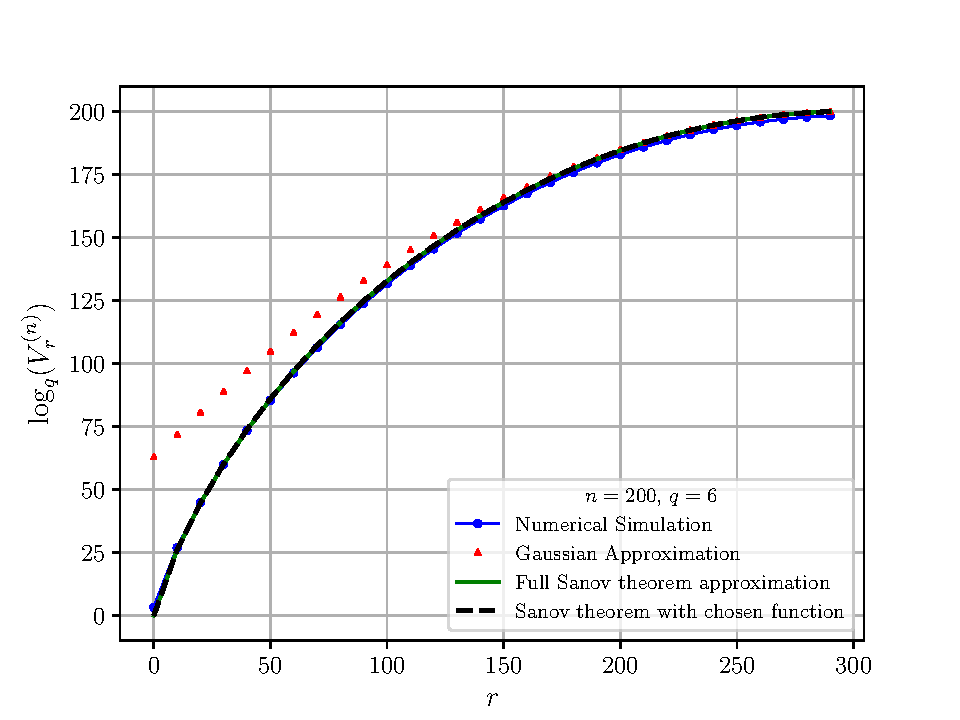
\includegraphics[width=0.5\textwidth]{myimage}
    \caption{Results of the Sanov theorem approximation compared to the actual value. Note the $\log$ scale on the $y$-axis. An approximation using the central limit theorem is also plotted for comparison. One can also see the near perfect match between the result of applying Sanov's theorem and the function defined.}
    \label{plot of approximations}
\end{figure}
\vspace*{-\baselineskip}
\begin{table}[htbp]
   % increase table row spacing, adjust to taste
   \renewcommand{\arraystretch}{1.3}
   \caption{Values of $c(q)$}
   \label{tab:table_example}
   \centering
   \begin{tabular}{|c|c|c|c|}
     \hline
     $q$ & $c(q)$ & $q$ & $c(q)$\\
     \hline
     $4$ & $6.7335$ & $10$ & $9.1297$\\
     \hline
     $5$ & $7.5202$ & $12$ & $9.8138$\\
     \hline
     $6$ & $7.6108$ & $15$ & $10.7921$\\
     \hline
     $7$ & $8.1711$ & $20$ & $12.1588$\\
     \hline
     $8$ & $8.3996$ & $25$ & $13.4049$\\
     \hline
     $9$ & $8.8682$ & $30$ & $15.5390$\\
     \hline
   \end{tabular}
\end{table}

\begin{figure}[htbp]
    \centering
    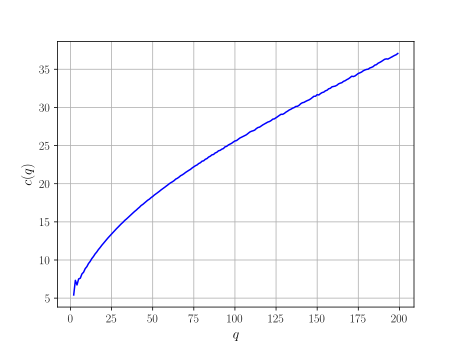
\includegraphics[width=0.5\textwidth]{cqwithq}
    \caption{Plot of $c(q)$ with respect to $q$}
    \label{fig:sim}
\end{figure}
\vspace{3mm}
\section{Bounds on the Lee metric}\label{Lee metric bounds}
Note that the results presented in the previous section imply that the volume of the Lee sphere of radius $pn$ is lower bounded by 
\begin{equation}\label{lee size}
    \log_q V_{pn}^{(n)} \geq n \left[1 + \frac{p \lambda(p) + \log \left(\sum_j \mathbb{P}_X(j) e^{-j \lambda(p)}\right)}{\log q}\right] - o(n)
\end{equation}
where $\lambda(p) = c(q)(\overline{D}^{\sfrac{1}{q}} - p^{\sfrac{1}{q}})$. There's also a very similar upper bound.
\begin{equation}
    \log_q V_{pn}^{(n)} \leq n \left[1 + \frac{p \lambda(p) + \log \left(\sum_j \mathbb{P}_X(j) e^{-j \lambda(p)}\right)}{\log q}\right] + o(n)
\end{equation}

We can use these bounds on the volume to find bounds on the possible rates of a code given the minimum distance criterion that the code must satisfy. We find such bounds in this section. 

\subsection{The Hamming Bound}
\iffalse
    \begin{lemma}[Hamming bound for a general metric]
    If a code has minimum distance $\delta n$, then $V_{\sfrac{\delta}{2}}^{(n)} \leq q^{n(1-R(\delta))}$, or 
    \begin{equation}
        R(\delta) \leq 1 - \frac{1}{n}\log_q(V_{\sfrac{\delta}{2}}^{(n)})
    \end{equation}
    \end{lemma}
    \begin{proof}
    The proof is given in \cite{Berlekamp:2015:ACT:2834146}, equation 13.11, and relies on a simple sphere packing argument.
    \end{proof}
\fi
\begin{theorem}[Hamming bound for the Lee metric] The rate $R(\delta)$ of a code in the Lee metric with minimum distance $\delta n$ is bounded above as
\begin{equation}
    R(\delta) \leq -\frac{\frac{\delta}{2} \lambda(\frac{\delta}{2}) + \log \left(\sum_j \mathbb{P}_X(j) e^{-j \lambda(\frac{\delta}{2})}\right)}{\log q} + o(1)
\end{equation}
\end{theorem}
\begin{proof}
The proof follows immediately by substituting $p = \frac{\delta}{2}$ in the expression for the bound on the volume of the Lee sphere (equation \cref{lee size}) and then using equation \cref{Hamming bound}.
\end{proof}

\subsection{The Gilbert-Varshamov Bound}
\iffalse
    \begin{lemma}[Gilbert-Varshamov bound for a general metric]
    Given blocklength $n$ and rate $R$, there is at least one code such that the minimum distance $d$ satisfies $V_d^{(n)} > q^{n(1-R)}$. The asymptotic version states that
    \begin{equation}
        R(\delta) \geq 1 - \frac{1}{n}\log_q(V_{\delta n}^{(n)})
    \end{equation}
    \end{lemma}
    \begin{proof}
    The proof is given in \cite{Berlekamp:2015:ACT:2834146}, theorem 13.71.
    \end{proof}
\fi
\begin{theorem}[Gilbert-Varshamov bound for the Lee metric] The optimal rate $R(\delta)$ of a code in the Lee metric with minimum distance $\delta n$ is bounded below as
\begin{equation}
    R(\delta) \geq -\frac{{\delta} \lambda(\delta) + \log \left(\sum_j \mathbb{P}_X(j) e^{-j \lambda(\delta)}\right)}{\log q} - o(1)
\end{equation}
\end{theorem}
\begin{proof}
The proof follows immediately by substituting $p = {\delta}$ in the expression for the bound on the volume of the Lee sphere (equation \cref{lee size}) and then using equation \cref{GV bound}.
\end{proof}

\subsection{The Elias-Bassalygo Bound}
\iffalse    
    \begin{lemma}[Elias-Bassalygo bound for a general metric]
    Given any rate $R$ and any $\epsilon > 0$, then for sufficiently large $n$,
    \begin{equation}
        \frac{d_{min}}{n} \leq \delta(R)\left[2 - \frac{\delta(R)}{\overline{D}}\right] + \epsilon 
    \end{equation}
    where $\delta(R)$ is the smallest solution of the equation $R = f(p)$ where $f(p) = 1 - \lim_{n \rightarrow \infty} \frac{\log_q(V_{pn}^{(n)})}{n}$
    \end{lemma}
    \begin{proof}
    The proof is given in \cite{Berlekamp:2015:ACT:2834146}, theorem 13.67.
    \end{proof}
\fi
Using the general form of the EB bounds given, for example, in \cite{Berlekamp:2015:ACT:2834146}, theorem 13.67, we get
\begin{theorem}[Elias-Bassalygo bound for the Lee metric] The rate optimal $R(\delta)$ of a code in the Lee metric with minimum distance $\delta n$ is bounded below as
\begin{equation}
    R(\overline{\delta}) \leq -\frac{{\overline{\delta}} \lambda(\overline{\delta}) + \log \left(\sum_j \mathbb{P}_X(j) e^{-j \lambda(\overline{\delta})}\right)}{\log q} + o(1)
\end{equation}
where $\overline{\delta} = \overline{D}\left(1 - \sqrt{1 - \frac{\delta}{\overline{D}}}\right)$
\end{theorem}

\begin{proof}
The proof follows after some simplification from the general expression and by substituting $p = \overline{\delta}$ in the expression for the bound on the volume of the Lee sphere (\cref{lee size}).
\end{proof}


\begin{figure}[htbp]
    \centering
    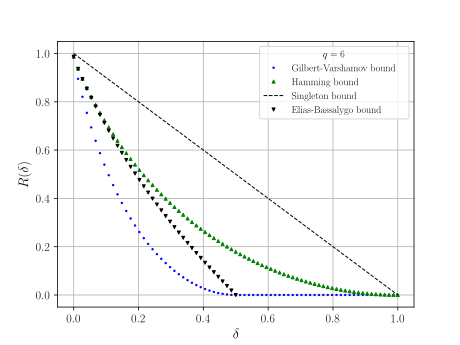
\includegraphics[width=0.5\textwidth]{bounds}
    \caption{The various bounds for the Lee metric. The Hamming, Gilbert-Varshamov and Elias-Bassalygo bounds are the results that we derive, and the singleton bound is from \cite{lee}. It is interesting to note that, like in the Hamming case, the singleton, the EB and GV bounds agree on the zero-rate point at $\delta = \overline{D}$. The EB bound is again the tightest upper bound.}
\end{figure}



%%%%%%
%% An example of a floating figure using the graphicx package.
%% Note that \label must occur AFTER (or within) \caption.
%% For figures, \caption should occur after the \includegraphics.
%%
% \begin{figure}[htbp]
%   \centering
%   \includegraphics[width=0.3\textwidth]{myfigure}
%   % where an .eps filename suffix will be assumed under latex,
%   % and a .pdf suffix will be assumed for pdflatex
%   \caption{Simulation results.}
%   \label{fig:sim}
% \end{figure}
%%%%%%

%%%%%%
%% An example of a double column floating figure using two subfigures.
%% (The subfigure.sty package must be loaded for this to work.)  The
%% subfigure \label commands are set within each subfigure command,
%% the \label for the overall figure must come after \caption.  
%% \hfil must be used as a separator to get equal spacing
%%
% \begin{figure*}[htbp]
%   \centerline{\subfigure[Case I]{\includegraphics[width=2.5in]{subfigcase1}
%       % where an .eps filename suffix will be assumed under latex,
%       % and a .pdf suffix will be assumed for pdflatex
%       \label{fig:first_case}}
%     \hfil
%     \subfigure[Case II]{\includegraphics[width=2.5in]{subfigcase2}
%       % where an .eps filename suffix will be assumed under latex,
%       % and a .pdf suffix will be assumed for pdflatex
%       \label{fig:second_case}}}
%   \caption{Simulation results.}
%   \label{fig:sim}
% \end{figure*}
%%%%%%

%%%%%%
%% An example of a floating table. 
%% Note that, for IEEE style tables, the \caption command should come
%% BEFORE the table. Table text will default to \footnotesize as IEEE
%% normally uses this smaller font for tables.  The \label must come
%% after \caption as always.
%%
% \begin{table}[htbp]
%   % increase table row spacing, adjust to taste
%   \renewcommand{\arraystretch}{1.3}
%   \caption{An Example of a Table}
%   \label{tab:table_example}
%   \centering
%   % Some packages, such as MDW tools, offer better commands for making tables
%   % than the plain LaTeX2e tabular which is used here.
%   \begin{tabular}{|c||c|}
%     \hline
%     One & Two\\
%     \hline
%     Three & Four\\
%     \hline
%   \end{tabular}
% \end{table}
%%%%%%


\section{Conclusion}
We have used Sanov's theorem and convex optimisation techniques to obtain estimates on the volume of a Lee ball and we then used it to obtain bounds on possible rates in the Lee metric. We now look at some possible directions of future work. Using the function $\lambda(p)$ that we defined, we were able to obtain a solution for the volume of a Lee sphere in terms of a summation. Whether we can obtain a closed form bound by possibly weakening it a little is still an open question. Also, the final convex optimisation problem in the case of the Lee metric is a maximisation over a single variable only, and as such should be solvable using calculus. However, the resulting equations are intractable. Also, we have included a plot that shows how well our function approximates the actual solution of that problem. We leave open the question of whether the solution of the equations obtained if we try to find the maxima by taking a derivative leads naturally to a function of the form we have used. 

Also, we have given Hamming and Gilbert-Varshamov bounds for the Lee metric. A bound analogous to the MRRW bound for the Lee metric remains open.

%%%%%%
%% Appendix:
%% If needed a single appendix is created by
%%
%\appendix
%%
%% If several appendices are needed, then the command
%%
% \appendices
%%
%% in combination with further \section-commands can be used.
%%%%%%


\section*{Acknowledgment}
We thank Prof Sidharth Jaggi of the Chinese University of Hong Kong (CUHK) for bringing bounds on the Lee metric to our attention and for several insightful discussions.

%%%%%%
%% To balance the columns at the last page of the paper use this
%% command:
%%
%\enlargethispage{-1.2cm} 
%%
%% If the balancing should occur in the middle of the references, use
%% the following trigger:
%%
%HAHAHAHAHHAHAHAHAHAH\IEEEtriggeratref{3}
%%
%% which triggers a \newpage (i.e., new column) just before the given
%% reference number. Note that you need to adapt this if you modify
%% the paper.  The "triggered" command can be changed if desired:
%%
%\IEEEtriggercmd{\enlargethispage{-20cm}}
%%
%%%%%%


%%%%%%
%% References:
%% We recommend the usage of BibTeX:
%%
\bibliographystyle{IEEEtran}
\bibliography{references}
%%
%% where we here have assume the existence of the files
%% definitions.bib and bibliofile.bib.
%% BibTeX documentation can be obtained at:
%% http://www.ctan.org/tex-archive/biblio/bibtex/contrib/doc/
%%%%%%


%% Or you use manual references (pay attention to consistency and the
%% formatting style!):


\end{document}


%%%%%%
%% Some comments about useful packages
%% (extract from bare_conf.tex by Michael Shell)
%%

% *** MISC UTILITY PACKAGES ***
%
%\usepackage{ifpdf}
% Heiko Oberdiek's ifpdf.sty is very useful if you need conditional
% compilation based on whether the output is pdf or dvi.
% usage:
% \ifpdf
%   % pdf code
% \else
%   % dvi code
% \fi
% The latest version of ifpdf.sty can be obtained from:
% http://www.ctan.org/pkg/ifpdf
% Also, note that IEEEtran.cls V1.7 and later provides a builtin
% \ifCLASSINFOpdf conditional that works the same way.
% When switching from latex to pdflatex and vice-versa, the compiler may
% have to be run twice to clear warning/error messages.


% *** CITATION PACKAGES ***
%
%\usepackage{cite}
% cite.sty was written by Donald Arseneau
% V1.6 and later of IEEEtran pre-defines the format of the cite.sty package
% \cite{} output to follow that of the IEEE. Loading the cite package will
% result in citation numbers being automatically sorted and properly
% "compressed/ranged". e.g., [1], [9], [2], [7], [5], [6] without using
% cite.sty will become [1], [2], [5]--[7], [9] using cite.sty. cite.sty's
% \cite will automatically add leading space, if needed. Use cite.sty's
% noadjust option (cite.sty V3.8 and later) if you want to turn this off
% such as if a citation ever needs to be enclosed in parenthesis.
% cite.sty is already installed on most LaTeX systems. Be sure and use
% version 5.0 (2009-03-20) and later if using hyperref.sty.
% The latest version can be obtained at:
% http://www.ctan.org/pkg/cite
% The documentation is contained in the cite.sty file itself.


% *** GRAPHICS RELATED PACKAGES ***
%
\ifCLASSINFOpdf
  % \usepackage[pdftex]{graphicx}
  % declare the path(s) where your graphic files are
  % \graphicspath{{../pdf/}{../jpeg/}}
  % and their extensions so you won't have to specify these with
  % every instance of \includegraphics
  % \DeclareGraphicsExtensions{.pdf,.jpeg,.png}
\else
  % or other class option (dvipsone, dvipdf, if not using dvips). graphicx
  % will default to the driver specified in the system graphics.cfg if no
  % driver is specified.
  % \usepackage[dvips]{graphicx}
  % declare the path(s) where your graphic files are
  % \graphicspath{{../eps/}}
  % and their extensions so you won't have to specify these with
  % every instance of \includegraphics
  % \DeclareGraphicsExtensions{.eps}
\fi
% graphicx was written by David Carlisle and Sebastian Rahtz. It is
% required if you want graphics, photos, etc. graphicx.sty is already
% installed on most LaTeX systems. The latest version and documentation
% can be obtained at: 
% http://www.ctan.org/pkg/graphicx
% Another good source of documentation is "Using Imported Graphics in
% LaTeX2e" by Keith Reckdahl which can be found at:
% http://www.ctan.org/pkg/epslatex
%
% latex, and pdflatex in dvi mode, support graphics in encapsulated
% postscript (.eps) format. pdflatex in pdf mode supports graphics
% in .pdf, .jpeg, .png and .mps (metapost) formats. Users should ensure
% that all non-photo figures use a vector format (.eps, .pdf, .mps) and
% not a bitmapped formats (.jpeg, .png). The IEEE frowns on bitmapped formats
% which can result in "jaggedy"/blurry rendering of lines and letters as
% well as large increases in file sizes.
%
% You can find documentation about the pdfTeX application at:
% http://www.tug.org/applications/pdftex


% *** MATH PACKAGES ***
%
%\usepackage{amsmath}
% A popular package from the American Mathematical Society that provides
% many useful and powerful commands for dealing with mathematics.
%
% Note that the amsmath package sets \interdisplaylinepenalty to 10000
% thus preventing page breaks from occurring within multiline equations. Use:
%\interdisplaylinepenalty=2500
% after loading amsmath to restore such page breaks as IEEEtran.cls normally
% does. amsmath.sty is already installed on most LaTeX systems. The latest
% version and documentation can be obtained at:
% http://www.ctan.org/pkg/amsmath


% *** SPECIALIZED LIST PACKAGES ***
%
%\usepackage{algorithmic}
% algorithmic.sty was written by Peter Williams and Rogerio Brito.
% This package provides an algorithmic environment fo describing algorithms.
% You can use the algorithmic environment in-text or within a figure
% environment to provide for a floating algorithm. Do NOT use the algorithm
% floating environment provided by algorithm.sty (by the same authors) or
% algorithm2e.sty (by Christophe Fiorio) as the IEEE does not use dedicated
% algorithm float types and packages that provide these will not provide
% correct IEEE style captions. The latest version and documentation of
% algorithmic.sty can be obtained at:
% http://www.ctan.org/pkg/algorithms
% Also of interest may be the (relatively newer and more customizable)
% algorithmicx.sty package by Szasz Janos:
% http://www.ctan.org/pkg/algorithmicx


% *** ALIGNMENT PACKAGES ***
%
%\usepackage{array}
% Frank Mittelbach's and David Carlisle's array.sty patches and improves
% the standard LaTeX2e array and tabular environments to provide better
% appearance and additional user controls. As the default LaTeX2e table
% generation code is lacking to the point of almost being broken with
% respect to the quality of the end results, all users are strongly
% advised to use an enhanced (at the very least that provided by array.sty)
% set of table tools. array.sty is already installed on most systems. The
% latest version and documentation can be obtained at:
% http://www.ctan.org/pkg/array

% IEEEtran contains the IEEEeqnarray family of commands that can be used to
% generate multiline equations as well as matrices, tables, etc., of high
% quality.


% *** SUBFIGURE PACKAGES ***
%\ifCLASSOPTIONcompsoc
%  \usepackage[caption=false,font=normalsize,labelfont=sf,textfont=sf]{subfig}
%\else
%  \usepackage[caption=false,font=footnotesize]{subfig}
%\fi
% subfig.sty, written by Steven Douglas Cochran, is the modern replacement
% for subfigure.sty, the latter of which is no longer maintained and is
% incompatible with some LaTeX packages including fixltx2e. However,
% subfig.sty requires and automatically loads Axel Sommerfeldt's caption.sty
% which will override IEEEtran.cls' handling of captions and this will result
% in non-IEEE style figure/table captions. To prevent this problem, be sure
% and invoke subfig.sty's "caption=false" package option (available since
% subfig.sty version 1.3, 2005/06/28) as this is will preserve IEEEtran.cls
% handling of captions.
% Note that the Computer Society format requires a larger sans serif font
% than the serif footnote size font used in traditional IEEE formatting
% and thus the need to invoke different subfig.sty package options depending
% on whether compsoc mode has been enabled.
%
% The latest version and documentation of subfig.sty can be obtained at:
% http://www.ctan.org/pkg/subfig


% *** FLOAT PACKAGES ***
%
%\usepackage{fixltx2e}
% fixltx2e, the successor to the earlier fix2col.sty, was written by
% Frank Mittelbach and David Carlisle. This package corrects a few problems
% in the LaTeX2e kernel, the most notable of which is that in current
% LaTeX2e releases, the ordering of single and double column floats is not
% guaranteed to be preserved. Thus, an unpatched LaTeX2e can allow a
% single column figure to be placed prior to an earlier double column
% figure.
% Be aware that LaTeX2e kernels dated 2015 and later have fixltx2e.sty's
% corrections already built into the system in which case a warning will
% be issued if an attempt is made to load fixltx2e.sty as it is no longer
% needed.
% The latest version and documentation can be found at:
% http://www.ctan.org/pkg/fixltx2e


%\usepackage{stfloats}
% stfloats.sty was written by Sigitas Tolusis. This package gives LaTeX2e
% the ability to do double column floats at the bottom of the page as well
% as the top. (e.g., "\begin{figure*}[!b]" is not normally possible in
% LaTeX2e). It also provides a command:
%\fnbelowfloat
% to enable the placement of footnotes below bottom floats (the standard
% LaTeX2e kernel puts them above bottom floats). This is an invasive package
% which rewrites many portions of the LaTeX2e float routines. It may not work
% with other packages that modify the LaTeX2e float routines. The latest
% version and documentation can be obtained at:
% http://www.ctan.org/pkg/stfloats
% Do not use the stfloats baselinefloat ability as the IEEE does not allow
% \baselineskip to stretch. Authors submitting work to the IEEE should note
% that the IEEE rarely uses double column equations and that authors should try
% to avoid such use. Do not be tempted to use the cuted.sty or midfloat.sty
% packages (also by Sigitas Tolusis) as the IEEE does not format its papers in
% such ways.
% Do not attempt to use stfloats with fixltx2e as they are incompatible.
% Instead, use Morten Hogholm'a dblfloatfix which combines the features
% of both fixltx2e and stfloats:
%
% \usepackage{dblfloatfix}
% The latest version can be found at:
% http://www.ctan.org/pkg/dblfloatfix


% *** PDF and URL PACKAGES ***
%
%\usepackage{url}
% url.sty was written by Donald Arseneau. It provides better support for
% handling and breaking URLs. url.sty is already installed on most LaTeX
% systems. The latest version and documentation can be obtained at:
% http://www.ctan.org/pkg/url
% Basically, \url{my_url_here}.



% *** Do not adjust lengths that control margins, column widths, etc. ***
% *** Do not use packages that alter fonts (such as pslatex).         ***
%%%%%%


%%% Local Variables:
%%% mode: latex
%%% TeX-master: t
%%% End:
